\chapter{Einleitung\label{Chapter1}}


\section{Motivation}

\TODO{cite REF REF}
Solides Testen im Web wird zunehmend zu einem der wichtigsten Bereiche in der Software Entwicklung sowie im Software Engineering. Um die Softwarequalit�t von Websites sicherzustellen, ist es essentiell anspruchsvolle Programme f�r die Testautomation zu entwickeln.

Das designen von Testf�llen ist eine entscheidende Testkomponente welche in hohem Ma�e die Qualit�t eines Tests bestimmt. Die Auswahl der Testf�lle legt den Grundstein f�r die Art sowie die Fokussierung des Tests.

Wenn Testf�lle auf Basis von Spezifikationen festgelegt werden, sind die daraus resultierenden Tests funktional. Funktionale Tests sind h�chst wichtig f�r die Verifikation von Software und werden von einer breiten Masse in der Industrie eingesetzt. Allerdings gibt es nur wenige Methoden und Applikationen welche die Systematische Erstellung von Testf�llen f�r funktionale Tests unterst�tzen. Deshalb wird h�ufig auf nur teilweise  anwendbare Tools zur�ckgegriffen, wie MS Excel oder Entscheidungstabellen.

Die Klassifikationsbaum-Methode ist eine effiziente Testmethode f�r funktionales testen, welche die M�glichkeit bietet, den kompletten Eingabebereich  eines Testobjekts in unabh�ngige �quivalenzklassen aufzuteilen.

\section{Zielsetzung}
Ziel dieser Arbeit ist es ein Java-Applikation zu entwickeln welche mit Hilfe von Klassifikationsb�umen automatisiertes Web Testing durchf�hrt. Web Testing beschreibt einen Teil des Softwaretestens, der sich auf Applikationen aus dem Web bezieht. 

Die Klassifikationsb�ume werden mit dem Programm Classification Tree Editor XL Professional von Berner \& Mattner\footnote{www.berner-mattner.com} erstellt.  Abbildung \ref{CTEXL} zeigt den CTE XL. Mit diesem Editor ist es weiterhin m�glich Testf�lle zu generieren. Die im CTE erstellten B�ume und generierten Testf�lle sollen in das Programm geladen werden und dort in verwendbare Java-Objekte gewandelt werden.

Mit Hilfe der Selenium WebDriver API f�r Java wird die Ansteuerung des Browsers automatisiert. Die API wirkt unterst�tzend bei der Kommunikation mit Webseiten, so dass auf diesen programmiertechnisch navigiert und interagiert werden kann.

Zur Ausf�hrung und Auswertung der Testf�lle werden JUnit Tests f�r die spezifischen vorgegebenen Websites entwickelt um automatisch, mit den Daten aus den zuvor erstellten Klassifikationsb�umen und der WebDriver API, die Tests auszuf�hren.

\begin{figure}[htbp]
\begin{center}
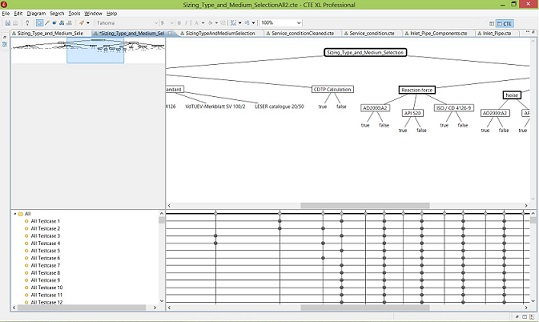
\includegraphics{./bilder/CTE_XL_BSP}
\caption{Classification Tree Editor XL}
\label{CTEXL}
\end{center}
\end{figure}

Im Endeffekt soll die Applikation dem Tester die Erstellung von Testf�llen erleichtern sowie die Ausf�hrung dieser automatisieren. Durch diese Vorteile reduziert sich der Testaufwand deutlich und erm�glicht eine effizientere Bearbeitung von Testobjekten.

\TODO{more more more, and ref}

\section{Gliederung}

\textbf{Kapitel \ref{Chapter1}}

Die Einleitung beschreibt die Motivation und Zielsetzung der Arbeit.

\textbf{Kapitel \ref{Chapter2}} 

Im zweiten Kapitel wird auf die Grundlagen f�r die Entwicklung des Programms eingegangen.

\textbf{Kapitel \ref{Chapter3}} 

Das dritte Kapitel analysiert die Anforderungen und behandelt das vorliegende Szenario.

\textbf{Kapitel \ref{Chapter4}} 
Dieses Kapitel behandelt die Implementierung und geht auf die Architektur sowie die Anwendung der Grundlagen ein.

\textbf{Kapitel \ref{Chapter5}} 

Kapitel f�nf beinhaltet die Fallstudie, es behandelt haupts�chlich die Anwendung des Programms auf das Test Objekt.

\textbf{Kapitel \ref{Chapter6}} 

Im Kapitel sechs wird ein Fazit gezogen und ein Ausblick gegeben.

\TODO{you know what}